\section{Mathematical background}
\label{sec:math}

% Singular Value Decomposition in general

Singular value decomposition (SVD) \cite{Baker2005, Kalman1996, Golub1996} is based on a theorem from linear algebra which says that a rectangular matrix $\mtrx{A} \in \mathbb{R}^{m \times n}$ can be decomposed into the product of three matrices - an orthogonal matrix $\mtrx{U} \in \mathbb{R}^{m \times m}$, a diagonal
matrix $\mtrx{S} \in \mathbb{R}^{m \times n}$, and the transpose of an orthogonal matrix $\mtrx{V} \in \mathbb{R}^{n \times n}$:

\begin{equation}
\mtrx{A} = \mtrx{U} \mtrx{S} \mtrx{V}^\mathsf{T},
\label{eq:svd-def}
\end{equation}

\noindent
where $\mtrx{U^\mathsf{T}U} = \mtrx{I}$, $\mtrx{V^\mathsf{T}V} = \mtrx{I}$; the columns of $\mtrx{U}$ are orthonormal eigenvectors of $\mtrx{AA^\mathsf{T}}$, the columns of $\mtrx{V}$ are orthonormal eigenvectors of $\mtrx{A^\mathsf{T}A}$, and $\mtrx{S}$ (sometimes referred to as $\mtrx{\Sigma}$) is a diagonal matrix containing singular values in descending order, which are at the same time the square roots of eigenvalues of $\mtrx{U}$ or $\mtrx{V}$.

SVD can be seen as a method for transforming correlated variables into a set of uncorrelated ones. At the same time, SVD is a method for identifying and ordering the dimensions along which data points show the most variation. Once it has been identified where the most variation is, it is possible to find the best approximation of the original data points using fewer dimensions. Hence, SVD can be seen as a method for data reduction/compression.

This is the basic idea behind SVD: taking a high dimensional, highly variable set of data points and reducing it to a lower dimensional space that exposes the substructure of the original data more clearly and orders it from most variation to the least. What makes SVD practical for data compression applications is that variation below a particular threshold can be simply ignored to massively reduce data with assurance that the main relationships of interest have been preserved.

The objective of a compression algorithm is to reduce amount of data representing FEM results and also the ability to reconstruct original data from its smaller representation. This saves storage capacity and also accelerates data transfer between computers as the analysis itself and the post-processing of results is usually done on different workstations.

Exact SVD of a $m \times n$ matrix has computational complexity $O(min(mn^2, m^2n))$ using the "big-O" notation. In \cite{Holmes2007, Candes2011, Woolfe2008, Martinsson2011} are described randomized algorithms for constructing approximate matrix factorizations that have better asymptotic complexity. Their main purpose is to accelerate calculations of matrix decompositions which tend to be very slow for large data sets.

Compression method can be lossy or lossless based on quality of data reconstructed from its compressed representation. Lossless methods are able to fully reconstruct original data. Lossy methods, on the other hand, produce only approximations of original data. 

SVD is used as part of the compression algorithm. SVD method applied to arbitrary matrix produces decomposition that consist of corresponding singular values and singular vectors. This process is fully reversible (with the assumption that the numerical errors are negligible). The original matrix can be reconstructed by the multiplication of decomposed parts. However, the compression algorithm is based on modification of decomposition to create low-rank approximation matrix. The reconstructed matrix slightly differs from the original matrix and algorithm therefore does lossy compression.

\subsection{Low-rank approximation matrix}

From the definition of SVD in (\ref{eq:svd-def}) and from the properties of SVD follows the fact that a matrix can be represented in the form of its SVD components as a sum of rank-1 matrices

%\begin{equation}
%\mtrx{A}=\mtrx{U_{1}}S_{1}\mtrx{V_{1}^{T}}+\mtrx{U_{2}}S_{2}\mtrx{V_{2}^{T}}+ ... +\mtrx{U_{n}}S_{n}\mtrx{V_{n}^{T}},
%\label{eq:svd-expansion}
%\end{equation}

\begin{equation}
\mtrx{A}=\sum_{i=1}^{n} s_{i}\bf{u}_i\bf{v}_i^{\mathsf{T}},
\label{eq:svd-expansion}
\end{equation}

\noindent
where $s_i$ is the $i$-th singular value, $\bf{u}_i$ and $\bf{v}_i$ are corresponding singular vectors, and $n$ is the rank of matrix~$\mtrx{A}$. Considering the fact that singular values are ordered $s_{1} \geq s_{2} \geq s_{3} \geq ... \geq s_{n}$, the above formula implies that the first term of the sum would have the highest contribution and the last term would have the lowest contribution to matrix~$\mtrx{A}$. Therefore, if we take only first $r$ members of the above summation we get an approximation matrix

%\begin{equation}
%\mtrx{A'}=\mtrx{U_{1}}S_{1}\mtrx{V_{1}^{T}}+\mtrx{U_{2}}S_{2}\mtrx{V_{2}^{T}}+ ... +\mtrx{U_{r}}S_{r}\mtrx{V_{r}^{T}}.
%\label{eq:svd-approx-expansion}
%\end{equation}

\begin{equation}
\mtrx{A'}=\sum_{i=1}^{r} s_{i}\bf{u}_i\bf{v}_i^{\mathsf{T}}.
\label{eq:svd-approx-expansion}
\end{equation}

The quality of approximation depends on the magnitude of the singular values omitted from the approximation formula, namely $s_{r+1} ...  s_{n}$. The compression algorithm is based on an assumption that the first singular value is order-of-magnitude higher than singular values at the end of the decomposition sequence. In special cases, when $r=n$ or $s_{i}=0$ for all $i \geq r$, the omitted singular values do not contribute to the sum and the compression is therefore lossless. In other cases, approximation error has to be calculated and taken into account to avoid loss of important details in data.

The main goal of the compression algorithm is to find a compromise between low approximation error and high compression ratio $c$ which is calculated using the formula

\begin{equation}
c=\frac{r(m+n+1)}{m n},
\label{eq:cr-def}
\end{equation}

\noindent
where $m$ and $n$ are dimensions of matrix $\mtrx{A}$. Explanation of the compression ratio formula is best done using Figure~\ref{fig:lowrank_svd}. Light color represents the part of matrix decomposition that is to be stored in the output file as a low-rank approximation of the input.

\begin{figure}[H]
\centering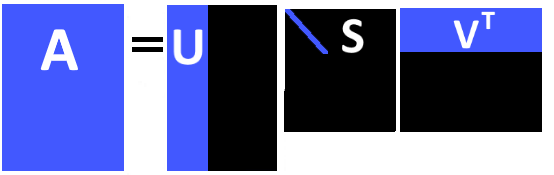
\includegraphics[width=0.7\textwidth]{figures/low_rank_decomposition_diagram}
\caption{Decomposition of input matrix $\mtrx{A}$ into diagonal matrix of singular values $\mtrx{S}$ and matrices of left and right singular vectors. Light color illustrates low-rank approximation.}
\label{fig:lowrank_svd}
\end{figure}

\subsection{Error estimation}
\label{sec:error}

The objective of data compression is to represent an input with smaller amount of data. However, the data reconstructed from its compressed representation may or may not be the exact copy of the original image. A compression technique can be lossy or lossless based on the quality of data it restores.

Low-rank approximation matrix method that is described in this paper is a lossy compression technique. Several error metrics are used to control the quality of results \cite{SairaBanu2015}.

\begin{itemize}
\item \textbf{Mean square error}
\begin{equation}
MSE=\frac{1}{m n} \sum_{i=1}^{m} \sum_{j=1}^{n} (A_{ij} - A'_{ij})^{2},
\label{eq:mse-def}
\end{equation}

\noindent
where $A_{ij}$ represents an element of the original matrix and $A'_{ij}$ represents an element of the
reconstructed matrix of dimension $m \times n$.

\item \textbf{Rooted Mean Square Deviation}
\begin{equation}
RMSD=\sqrt{MSE}.
\label{eq:rmsd-def}
\end{equation}

\item \textbf{Normalized Rooted Mean Square Deviation}
\begin{equation}
NRMSD=\frac{RMSD}{X_{max}-X_{min}}=\frac{\sqrt{MSE}}{X_{max}-X_{min}},
\label{eq:nrmsd-def}
\end{equation}

\noindent
where $X_{min}$ and $X_{max}$ are elements of input matrix $\mtrx{A}$ with minimum and maximum value, respectively. This error metric is able to measure and compare errors in datasets with different scales. Therefore, it is the main parameter that is used to control the quality of compression in the algorithm presented in this paper.

\item \textbf{Peak Signal to Noise Ratio}

PSNR is most commonly used to measure the quality of reconstruction of lossy compression methods (e.g. image compression). The signal in this case is the original data, and the noise is the error introduced by compression. PSNR is an approximation to human perception of reconstruction quality. This metric is not so important in area of FEM analyses, where the human perception of visualizations is not as important as the exact mathematical accuracy of approximations. The reason to include PSNR in results is in particular to allow comparison with other image-related compression methods. PSNR is usually expressed in terms of the logarithmic decibel scale (dB)

\begin{eqnarray}
PSNR &=& 10\log_{10}\frac{(X_{max}-X_{min})^{2}}{MSE} =
\\
&=& 20\log_{10}\frac{X_{max}-X_{min}}{\sqrt{MSE}}=20\log_{10}\frac{1}{NRMSD} = \nonumber
\\
&=& -20\log_{10}NRMSD. \nonumber
\label{eq:psnr-def}
\end{eqnarray}

\end{itemize}

%%%%%%%%%%%%%%%%%%%%%%%%%%%%%%%%%%

%\subsection{Randomized SVD}
%In \cite{Holmes, Halko2011, Candes2009} are described randomized algorithms for constructing approximate matrix factorizations. Their main purpose is to accelerate calculations of matrix decompositions which tend to be very slow for large data sets.

%Exact SVD of a $m \times n$ matrix has time complexity $O(min(mn^2, m^2n))$ using the "big-O" notation. Assume the data points are in the columns of $\mtrx{A} \in \mtrx{M_{m,n}}(\mathbb{R})$ where $m \leq n$. Note that $\mtrx{AA^T}$ is the dataset covariance matrix. Then a simple method is to randomly choose $k<m$ columns of $\mtrx{A}$ that form a matrix $\mtrx{B}$. Statistically, the SVD of $\mtrx{BB^T}$ will be close to that of $\mtrx{AA^T}$; thus it suffices to calculate the SVD of $\mtrx{B}$, the complexity of which, is only $O(k^2m)$.

% http://mathoverflow.net/questions/161252/what-is-the-time-complexity-of-truncated-svd

%%%%%%%%%%%%%%%%%%%%%%%%%%%%%%%%%%


% subsection: Sparse matrix of details: Mozna uplne vyhodit, stejne to neni implementovano -- uvest jen v sekci Optimization nebo v Conclusion
